\documentclass[9pt]{article}
\usepackage[textwidth=13cm,textheight=19.5cm]{geometry}
\usepackage{changepage}
\usepackage{graphicx, verbatim, lipsum, layouts, listings, minted, framed,
fancyhdr, titlesec, soul, color}

\pagestyle{fancy}
\fancyhf{}
\fancyhead[L]{\rightmark}
\fancyhead[R]{\thepage}
\fancyfoot[CE,CO]{\thepage}
\renewcommand{\headrulewidth}{0pt}
\usemintedstyle{pastie}

\DeclareRobustCommand{\hlgreen}[1]{{\sethlcolor{green}\hl{#1}}}

\title{
	Development Stage\\
	\large{HND Graded Unit}\\
}
\author{Colin J. Barr}
\date{}

\renewenvironment{framed}[1][\hsize]
   {\MakeFramed{\hsize#1\advance\hsize-\width \FrameRestore}}%
   {\endMakeFramed}

\begin{document}

\maketitle
\tableofcontents{}

\section{Production}
	\subsection{Problem domain}
		\subsubsection{Visitor pattern}
			jAudit utilises a visitor pattern to traverse the AST in order to
			yield nodes from it. Most notably, the \textit{MethodTreeVisitor}
			class visits \textit{MethodDeclaration} nodes and appends them to
			the root - class - node.

			\begin{framed}[1.2\textwidth]	
				\begin{minted}[linenos]{java}
/**
 * Method-visitor designed for appendage to method-tree
 */
public class MethodTreeVisitor extends VoidVisitorAdapter<ClassTreeNode> {

    /**
     * Visit AST method
     * @param methodDecl method declaration node
     * @param root tree node being appended to (where the methods are leaves)
     */
    @Override
    public void visit(MethodDeclaration methodDecl, ClassTreeNode root) {
	// ensure relevant siblings are traversed by adapter (parent)
        super.visit(methodDecl, root); 
        // add method to root node
        root.add(new MethodTreeNode(methodDecl));
    }

}
				\end{minted}
			\end{framed}

			The above visitor is responsible for populating the method tree
			which used used as a primarily navigational and informative
			component.

			\begin{figure}[H]
				\centering
				\includegraphics[width=0.35\textwidth]{res/method-tree.png}
				\caption{Method tree component populated with visitor}
			\end{figure}

			The visitor itself is extending an \textit{adapter} because the
			\textit{VoidVisitorAdapter} allows subclasses to access its super
			methods which correctly implement node traversal for all nodes in
			the AST. Thus, one can isolate specific node(s) as I have done here.

		\subsubsection{Migrations}
			jAudit uses a database for efficient storage of audits (and
			references to the file(s) the audit(s) reference). Since jAudit must
			create the SQLite tables it requires on the user's machine, I chose
			to create a system somewhat similar to how Laravel manages database
			revisions. I opted to create an elementary \textit{migrations}
			system. Each migration simply contains logic required to \textit{up}
			(construct) and \text{down} (reverse) creational aspects of the
			database. For example, there exists a migration for the creation of
			both the audit and file table.\\

			The blueprint for a migration can be seen below:\\

			\begin{framed}[1.2\textwidth]	
				\begin{minted}[linenos]{java}
/**
 * Migrations allow for the easy creation and destruction of database schemas.
 */
public abstract class Migration {
    protected DBConnection connection;

    /**
     * Common constructor for dependency injection of database connection
     *  (see {@link DBConnection}) for easier testing.
     *
     * @param connection dependency injectable connection to be used
     * by the migration
     */
    public Migration(DBConnection connection) {
        this.connection = connection;
    }

    /**
     * The method is for creational actions upon the database schema.
     *
     * @return whether the migration was completed successfully
     */
    public abstract boolean up();

    /**
     * The method is for reversing the actions of {@link Migration#up()}.
     *
     * @return whether the migration's reversal was completed successfully
     */
    public abstract boolean down();
}
				\end{minted}
			\end{framed}

			As you can see, the Migration itself is an \textit{abstract} class,
			therefore one can't instantiate it itself. One must instantiate a
			subclass concretion that implements the abstract methods
			\texttt{up()} and \texttt{down()}.\\

			It's also worth noting that the Migration class has a constructor
			that sets a \textit{protected} \texttt{DBConnection}. This is to
			allow for \textit{dependency injection} so that the migrations can
			operate on independent connections and be easier to test since we
			can also supply them with \textit{facade} connections purely for
			debugging.\\

			The actual depedency-injectable \texttt{DBConnection} class is a
			\textit{singleton} class that acts a minimal wrapper around a
			\texttt{java.sql.Connection}.\\

		\subsubsection{Serializer}
			
			In order to prepare the context of an audit for storage in a
			database, the audit context must be tranposed to a JSON
			representation.\\

			I use Google's JSON library, GSON, to do this. GSON allows you to
			register an adapter-serializer for custom types. I decided to
			implement a serializer for the audit context that would consist of
			the root node (with its content) and all children nodes (without
			content) and their positions. Only the root node's content is stored
			because it would be redundant to store extra content already
			contained within the root node.\\

			The user \textit{reduces} an audit by simply selecting a range of
			adjacent nodes in a context-trace from the auditor view (shown
			below).\\

			\begin{figure}[H]
				\centering
				\includegraphics[width=0.5\textwidth]{res/context-select.png}
				\caption{Selecting relevant context via reduction}
			\end{figure}
			
			The above context reduction gets tranposed to:\\

			\begin{framed}[1.2\textwidth]
				\begin{minted}[linenos]{json}
{
  "IfStmt": "if (tw !\u003d null) {\n    tw.activate(null, false);\n}",
  "children": [
    ["BlockStmt", [802, 25], [804, 9]],
    ["ExpressionStmt", [803, 11], [803, 35]],
    ["MethodCallExpr", [803, 11], [803, 34]],
    ["BooleanLiteralExpr", [803, 29], [803, 33]]
  ]
}
				\end{minted}
			\end{framed}

		\subsubsection{Multithreading}

			jAudit utilises multi-threading during its parsing stage because the
			time that parsing each file could potentially take isn't exactly
			deterministic. Thus, in order to avoid blocking the GUI thread when
			parsing, it's executed in the background; in another thread. 

			\begin{framed}[1.2\textwidth]	
				\begin{minted}[linenos]{java}
private class ParserWorker extends SwingWorker<Boolean, Boolean> {

@Override
protected Boolean doInBackground() throws ParseProblemException {
	// attempt to parse file
	parsedFile = initCompilationUnit();

	// if parsing is successful, run method visitor to initialise method-tree
	if (parsedFile) {
		initTree();
	}

	// if parsing failed without throwing ParseProblemException,
	// return success value anyway
	return parsedFile;
}

/**
 * Parsing complete callback, closes progress dialog.
 */
@Override
protected void done() {
	// queue progress-dialog closure in AWT event queue
	SwingUtilities.invokeLater(() -> showProgressDialog(false));

	// state
	try {
		parsedFile = get();
	} catch (InterruptedException | ExecutionException e) {
		e.printStackTrace();
	}
}
}
				\end{minted}
			\end{framed}

		\subsubsection{Audit Report Output}
			Another aspect of the problem domain is the ability to output audit
			reports from jAudit which outputs reports such as the following:\\

			\begin{figure}[H]
				\centering
				\includegraphics[width=\textwidth]{res/audit-report.png}
				\caption{Example audit report output}
			\end{figure}

	\subsection{UI domain}
		\subsubsection{Layout}
			
			All of jAudit's \textit{views} (GUI) were written by-hand using Java
			Swing so I was required to pay extra detail to how I laid components
			out as to retain layout proportions whilst providing a versatile
			layout. 

			An example of how I managed to retain proportions is shown below:\\

			\begin{figure}[H]
				\centering
				\includegraphics[width=\textwidth]{res/comparison.png}
				\caption{Small and large layout from resizing}
			\end{figure}

			To make such a proportional layout possible whilst retaining layout
			versatility, I opted to wrap the major graphical components of the
			audit pane into splitpanes. The user can adjust the splits as they
			like.\\

			On top of this, a visualisation component I created - the graph view
			- can also be dragged around using mouse drags to increase
			  accessibility as it can be annoying to click precisely on
			  scrollbars. Thus, you can scroll the graph view by simply
			  dragging. That aspect of the graph view is also highlighted below.\\

			\begin{figure}[H]
				\centering
				\includegraphics[width=.8\textwidth]{res/split.png}
				\caption{Splits and draggable area highlighted}
			\end{figure}


		\subsubsection{Navigation}

			As described in the project planning stage, the method tree is not
			only a component designed for an overview of the parsed class'
			method(s), it also is designed to act as a navigational component.
			By simply selecting any method, the source view will jump to that
			method's declaration and centre it in the view.\\

			\begin{figure}[H]
				\centering
				\includegraphics[width=\textwidth]{res/navigation.png}
				\caption{Depiction of on-select navigation and method centering}
			\end{figure}

			The method gets centred so that any methods that are navigated to
			that exist below the current view don't get shown on the last line
			of the source view as this would require the user to manually scroll
			down further to actually see the method's implementation.\\
			
		\subsubsection{Graph view}
			
			In jAudit's planning stage and proposal, there's lots of elements of
			visualisation to help the reader understand what the meaning of "AST
			context-depth", etc. is. I decided that it'd be interesting to
			create a \textit{custom component} for visualisation purposes. So I
			opted to create a graph view that displays the AST context-depth as
			a directed-acyclic graph with an in/out degree or 0 or 1 (sort of
			like a singly linked list being visualised).\\

			That endeavour resulted in the component below being created:\\

			\begin{figure}[H]
				\centering
				\includegraphics[width=\textwidth]{res/drag.png}
				\caption{Draggable graph view custom component}
			\end{figure}

			It was evident that such a component that could potentially produce
			graphs that wouldn't be able to be fully visible on smaller screens
			would require some form of scrolling. So I wrapped it in a
			scrollable pane and then implemented the ability to click and drag
			the graph around.\\

			I consider the ability to drag it an aid to both the user experience
			and accessibility of the program. It feels a lot more fluid to just
			grab and drag the view rather than manually scroll with the
			scrollbars (which requires a certain degree of precision when
			clicking - such a precision that may be taxing for disabled users
			with a disease such as Parkinson's).\\

			The class hierarchy for this custom component is shown below:\\

			\begin{figure}[H]
				\centering
				\includegraphics[width=\textwidth]{res/graph-hierarchy.png}
				\caption{Graph class hierarchy}
			\end{figure}

		\subsubsection{Localisation}

			jAudit also supports the German language as parts of its
			localisation support. The choice to support German stemmed from my
			own recreational learning of German to converse with online
			friends.\\

			Upon starting jAudit, the user is prompted to choose a language
			using the dialog depicted below. Of course, the dialog currently
			only supports (British) English and (High) German.\\

			\begin{figure}[H]
				\centering
				\includegraphics[width=0.4\textwidth]{res/lang-select.png}
				\caption{Language selection dialog}
			\end{figure}

			An example of the audit view in localised German is shown below:\\

			\begin{figure}[H]
				\centering
				\includegraphics[width=0.9\textwidth]{res/german.png}
				\caption{jAudit with German localisation}
			\end{figure}

		\subsubsection{Gutter Audit Tooltip}

			When an audit is created (or loaded from a database), its location
			is bookmarked in the gutter of the text view component displaying
			the source file. This annotation icon provides the audit comment as
			its tooltip to allow the user to easily see what's audited at
			certain source code locations.\\

			\begin{figure}[H]
				\centering
				\includegraphics[width=0.7\textwidth]{res/gutter.png}
				\caption{Gutter bookmark with audit comment as tooltip}
			\end{figure}

		\subsubsection{Drag \& Drop Opening}
			
			In order to aid the user experience, I implemented the ability to
			drag \& drop files into jAudit's window to open them. I believed
			this would make opening files somewhat more efficient and practical
			if the user has a file manager currently open and knows what file
				they want to open. 

	\subsection{Unfamiliar libraries}
		Many unfamiliar libraries were used in this project. I used the
		\textit{Maven}
		management system to manage dependencies within the project. Such
		dependencies are listed below.
		
		\subsubsection{JavaParser}
			As noted in the project planning stage, the business logic in
			jAudit relies heavily on the parsing functionality of JavaParser
			which is used to construct an AST from given source files. jAudit
			then traverses this AST to map arbitrary audit comments to reduced
			ranges within the AST. This allows for construct-relative
			contextual auditing.\\

			The choice to use \textit{JavaParser} was made just before the project was
			assigned so using it was actually quite a risk. A few design
			decisions made in JavaParser caused a few minor hinderences during
			development. For example, I discovered a few bugs that I've since
			reported. These were rather obscure bugs such as JavaParser's
			compilation unit appending newline characters to the end of (this
			behaviour isn't defined so it caused a few issues with mapping
			source code to the AST because every selection was, as a result,
			offset from where it really is in the source file by the number of
			fields existent in a class). Another nuance is the way JavaParser
			doesn't really bother with any parsing of comments. This may seem
			like a good idea since parsers ignore comments (e.g. the entire
			point of comments), but it actually causes nodes after comments'
			contents to start with comments which isn't the most useful
			feature.

		\subsubsection{GSON}
			Google's \textit{GSON} project is used to serialize the audit-context to
			JSON for storage purposes. I considered a hacky approach like
			Java's own object serialization but favoured the JSON format for
			portable practicality, storage, better standardisation, faster
			parsing, etc.

		\subsubsection{WebLaf}
			\textit{WebLaF} is a LaF (Look and Feel) used for the styling of Java Swing
			components. I opted to use it because I thought it was visually
			appealing in comparison to alternatives. It also provides lots of
			useful tailor-made components (only one of which I used - the
			memory bar in the status bar).  

		\subsubsection{j2html}
			\textit{j2html} was used in order to make the generation of HTML
			(for the reports) more idiomatic. The expressive way that you can
			describe how a HTML document should be rendered (in terms of DOM)
			improves the maintainability and readability of the code. 

		\subsubsection{RSyntaxTextArea}
			\textit{RSyntaxArea} is a custom component I used for the display of
			syntax-highlighted source code within a text-area. I chose it
			because implementing syntax-highlighting from scratch would simply
			result in creating the wheel. There's no practical reason to
			reinvent the wheel when a mature project such as RSyntaxArea
			exists.
		
		\subsubsection{Dependency Tree}
			
			The dependency tree for all of these additional libraries can be
			seen below:
			
			\begin{framed}[1.3\textwidth]
				\begin{figure}[H]
					\centering
					\includegraphics[width=\textwidth]{res/dependencies.png}
					\caption{Dependency Tree}
				\end{figure}
			\end{framed}

	\subsection{Error handling}
		\subsubsection{GitHub URL verifier}
			jAudit supports a feature to open files from GitHub repository
			URLs. I implemented input validation for this as a first line of
			defence against invalid input. This involved creating a custom
			verifier class that verified the \textit{form} of the URL (e.g. the
			structure - no check that the remote resource exists is performed
			until the file's download is attempted). It parses it as a URL and
			makes sure it's in valid form. The verifier itself is a form of
			\textbf{error prevention} because it's not possible to submit the
			URL until it's confirmed as valid by the verifier (that's bound to
			the input field). Until the input is valid, the view highlights the
			input field as red (to signify invalidity) and disables the "Load"
			button.\\

			This restriction on the GUI as a the form of error prevention can
			be seen below:\\

			\begin{figure}[H]
				\centering
				\includegraphics[width=0.5\textwidth]{res/git-invalid.png}
				\caption{Invalid input with input prompt showing}
			\end{figure}

			\begin{figure}[H]
				\centering
				\includegraphics[width=0.5\textwidth]{res/git-invalid-text.png}
				\caption{Invalid input with "Load" button disabled}
			\end{figure}

			\begin{figure}[H]
				\centering
				\includegraphics[width=0.5\textwidth]{res/git-valid.png}
				\caption{Valid input with enabled "Load" button}
			\end{figure}

			A unit test that employs the verifier used by the view above is also
			documented in the testing section.

		\subsubsection{GitHub directory validation}
			
			When downloading a file from GitHub using the feature described in
			the previous section, the user is prompted to select a directory to
			save the file. Input validation was required here because the
			directory the user selects could potentially be outwith the
			permissions of the user. For example, on Linux, the default user
			group doesn't have \textit{write access} to \texttt{/usr/lib/}.
			Attempting to do so would cause a \textit{Permission denied} error.
			Similarly, an Exception of that nature would be thrown in Java if
			you attempted to write to a File that references a directory that
			the user doesn't have permissions for.\\

			I handled the above situation by using a loop that notifies the
			user of the invalid nature of their directory selection and then
			continually prompts them to re-input the directory. On top of this,
			I allowed the user to retain the ability to simply \textit{Cancel}
			the entire action safely.


			\begin{figure}[H]
				\centering
				\includegraphics[width=\textwidth]{res/boot-dir.png}
				\caption{Selection of directory default user has insufficient
				permissions for (\texttt{/boot/EFI/boot})}
			\end{figure}

			\begin{figure}[H]
				\centering
				\includegraphics[width=0.7\textwidth]{res/permissions.png}
				\caption{Error prompt shown to notify user of contained error}
			\end{figure}

		\subsubsection{Parse problem view}

			In the early stages of the project, any errors encountered during
			JavaParser's parsing would result in an undescriptive error message
			being shown. However, after reconsidering the target-demographic of
			this project, and knowing that I'd personally find useless
			information incredibly vexing, I decided to implement a rather
			rudimentary error view for error resolution.

			When a file can't be parsed due to parser errors, the dialog below is
			shown and the user can optionally choose to view the errors.\\

				\begin{figure}[H]
					\centering
					\includegraphics[width=\textwidth]{res/parse-error.png}
					\caption{Error message shown when file can't be parsed}
				\end{figure}

				\begin{figure}[H]
					\centering
					\includegraphics[width=\textwidth]{res/parse-error-view.png}
					\caption{Error prompt shown to notify user of contained error}
				\end{figure}
			
			Granted, the errors highlighted aren't the most helpful but, as noted,
			jAudit is targeted at expert users (the developers considered skilled
			enough to audit other peoples' code) so this feature certainly isn't
			the crux of error resolution within the project.

		\subsubsection{Checksum warning}

			In order for jAudit's source-relative audits to retain their source
			validity, it should be noted that jAudit's files must be treated as
			immutable once they're inserted.\\

			For this reason, checksums for files are calculated each time
			they're loaded. If an entry for the loaded file already exists, a
			checksum comparison is performed. If the checksums don't match, it
			implies the file has been modified since it was originally inserted
			into the database. Thus, the user is warned of this.\\

			\begin{figure}[H]
				\centering
				\includegraphics[width=\textwidth]{res/checksum.png}
				\caption{Checksum warning prompt}
			\end{figure}

			Above you can see the prompt shown to the user upon the loading of a
			modified file. jAudit will still attempt to emplace bookmarks for
			the loaded file with the offsets previously stored. However, any
			audits that can't be mapped are simply suppressed.\\

			I consider this a leniant form of error prevention as it notifies
			the user and, given the demographic of the program, the ability to
			attempt to continue to map audits seems suitable.\\

			\subsubsection{Custom Exception}

				I implemented a custom exception that is thrown when a user
				attempts to reduce an audit context to an invalid range. A valid
				range must extend a minimum of two nodes. A range consisting of
				a single-selected node is invalid.\\

				\begin{framed}[1.2\textwidth]	
					\begin{minted}[linenos]{java}
package org.colin.exceptions;

/**
 * Exception thrown when selected node ranges are invalid.
 */
public class InvalidNodeRangeException extends Exception {
    /**
     * Construct invalid node range exception with message
     * @param message exception message
     */
    public InvalidNodeRangeException(final String message,
	                                 final int first, final int last) {
        super(message + " " + first + " -> " + last);
    }
}
					\end{minted}
				\end{framed}

				An example where this is implemented is shown below:
				
				\begin{framed}[1.2\textwidth]	
					\begin{minted}[linenos]{java}
/**
 * Reduce model's context using sub-listing of an ordered-pair range
 *
 * @param first first index
 * @param last  last index
 * @throws InvalidNodeRangeException if reduction range is invalid, this is thrown
 */
public void reduceContext(int first, int last) throws InvalidNodeRangeException {
	if (first == last)
		throw new InvalidNodeRangeException("Node range must extend
		                                     two nodes", first, last);

	// sublist context
	context.sublist(first, last);
}
					\end{minted}
				\end{framed}


		
	\subsection{Internal documentation}

		All of jAudit is internally documented using JavaDoc. By taking this
		approach to documentation, I was able to quickly return to the project
		after breaks from working on it. JavaDoc also allowed me to easily
		generated documentation comprising the documentation comments I wrote
		for everything within the project.\\

		I also spent a few minutes adjusting the default stylesheet provided by
		JavaDoc to my liking. Examples of such JavaDoc generated output can be
		seen below:\\ 

		\begin{figure}[H]
			\centering
			\includegraphics[width=\textwidth]{res/docs.png}
			\caption{Extract from index page of documentation}
		\end{figure}

		I also attempted to document the package overview to make the resultant
		documentation a lot easier to navigate.\\

		\begin{figure}[H]
			\centering
			\includegraphics[width=.6\textwidth]{res/package.png}
			\caption{Package documentation}
		\end{figure}

		As alluded to, the inline documentation was also aided by my choice of
		IDE that allowed me to practically view documentation without having to
		navigate to another file or open the documentation in my browser.\\

		\begin{figure}[H]
			\centering
			\includegraphics[width=.7\textwidth]{res/inline-docs.png}
			\caption{Inline documentation in IntelliJ IDEA}
		\end{figure}

	\subsection{Version control}

		In order to keep track of developmental changes within the project, I
		opted to use the \textbf{git} version control system. Git allowed me to
		effectively manage revisions within the project.\\

		At first, git wasn't used often because I was busy creating the initial
		beginning of the project so any changes were inherently minor. However,
		as development progressed and the source code base became harder to
		manage, git became an invaluable asset to me. I also chose to use the
		popular online git repository website github to backup my project.\\

		By looking at the git commits, one can see how the project developed
		over time and when specific features were implemented. This gives
		anyone intent on committing to the project a better idea of how the
		project grew over time. 

		\begin{figure}[H]
			\centering
			\includegraphics[width=\textwidth]{res/git.png}
			\caption{List of commits}
		\end{figure}

		Luckily, the IDE I used for the development of jAudit - IntelliJ IDEA -
		supported git integration out-of-the-box. This made using git to manage
		the project correctly incredibly practical and easy.
		
		\begin{figure}[H]
			\centering
			\includegraphics[width=0.8\textwidth]{res/idea-git.png}
			\caption{IntelliJ IDEA's \textit{git} Feature}
		\end{figure}

\section{Testing}

	\subsection{Cross platform}
		Since jAudit is written in Java, it should be able to run on all major
		operating systems such as Windows, Mac, and mainstream Linux
		distributions.\\

		I tested the functionality of jAudit on both Linux \& Windows.\\

		\begin{figure}[H]
			\centering
			\includegraphics[width=0.9\textwidth]{res/windows-jaudit.png}
			\caption{jAudit running under Windows}
		\end{figure}

		\begin{figure}[H]
			\centering
			\includegraphics[width=0.9\textwidth]{res/linux-jaudit.png}
			\caption{jAudit running under Linux}
		\end{figure}

	\subsection{Profiling}

		In choosing Java as the development language of jAudit, I knew I'd
		have concerns over the JVM's notorious memory usage. In order to
		gain metrics regarding these worries, I decided to profile the JVM
		during the execution of a usual jAudit session.\\

		For context, the JVM version used is shown below:

\begin{lstlisting}
> $ java -version
openjdk version "1.8.0_144"
OpenJDK Runtime Environment (build 1.8.0_144-b01)
OpenJDK 64-Bit Server VM (build 25.144-b01, mixed mode)
\end{lstlisting}

		\subsubsection{Heap Overview}

			Ever since the inception of jAudit, I was adamant on the JVM memory
			usage component that you can see at the bottom of the main window's
			status bar. After seeing how memory usage seemed to fluctuate whilst
			performing different actions from within jAudit, I decided to see
			how the heap responded to the opening and parsing of files.\\

			The graph below shows how the JVM heap memory fluctuated during the
			opening and parsing of 2 files in the one session:\\

			\begin{figure}[H]
				\centering
				\includegraphics[width=0.9\textwidth]{res/profiling/heap-resize.png}
				\caption{Heap fluctuation caused by parsing 2 files}
			\end{figure}

			As you can see, it's easy to work out when the two files were
			loaded. The two major spikes in the \textit{Used Heap} show the
			sharp heap usage used by the parsing stage of jAudit. The first
			spike also noticeably shows how the \textit{Heap Size} resizes to
			accomodate the spikes in heap usage. This extra allocated JVM heap
			memory acts as a safety net to avoid the JVM crashing with a
			\texttt{java.lang.OutOfMemoryError} exception.\\
			
			I suspect that the JVM internally allocates this extra heap memory -
			the safety net - relative to the growth of used heap memory over
			time. This would explain why the JVM heap retains its rather
			excessive size long after the two spikes have occured; e.g. if the
			JVM experiences a sharp increase in non-deterministic heap
			allocations, it will allocate an excessive heap size so it doesn't
			have to continually resize its own heap to account for volatile
			spikes in usage. 

		\subsubsection{Largest Objects}
			
			Another metric that I believed would be quite interesting - given
			the amount of dependencies used in jAudit - were the largest objects
			allocated by each part of the program. I believed this metric would
			provide keen insight into the overhead caused by certain jAudit
			dependencies.\\

			A part of jAudit that I suspected would have significant overhead
			instinctively - and partially after seeing the redraw lag on
			resizing the main window - is the look and feel provided by
			\textit{WebLookAndFeel}.\\

			WebLookAndFeel provides the look and feel used by jAudit - and a few
			of the components used. To work out the overhead imposed by this
			dependency, I used VisualVM to query the largest 20 objects related
			to the \textit{MainView} context. The result of this query is
			shown below:\\

			\begin{figure}[H]
				\centering
				\includegraphics[width=0.9\textwidth]{res/profiling/biggest-objects.png}
				\caption{Largest objects used by the \textit{MainView} instance}
			\end{figure}
			
			The objects I consider relevant, listed by order of size, are
			tabulated below:\\

			\begin{center}
			\begin{tabular}{ |p{10cm}|p{3cm}|  }
				\hline
				\multicolumn{2}{|c|}{Relevant \texttt{MainView} Overhead} \\
				\hline
					Instance Name & Size (bytes)\\
				\hline
					\texttt{com.alee.skin.web.WebSkin} & 3,217,603\\
					\texttt{com.alee.managers.style.data.SkinInfo} & 3,217,579\\
					\texttt{com.alee.managers.language.LanguageManager} &
					975,597\\
					\texttt{org.fife.ui.rsyntaxtextarea.modes.JavaTokenManager}
					& 789,572 \\
				\hline
			\end{tabular}
			\end{center}

			From the table above, one can conclude that WebLookAndFeel is an
			expensive dependency to have on jAudit as it takes up more than 6
			megabytes when idle (all \texttt{com.alee.*} are WebLaF packages).
			Another, reasonably large, source of overhead comes from the
			\texttt{org.fife.ui.*} packages as they're responsible for providing
			the syntax-highlighting text component used for displaying code in
			jAudit.

		\subsubsection{Object Querying}

			Given the - admittedly nondescript - overview seen in the previous
			sections, I decided it would be interesting to query specific
			objects using the JVM's OQL (Object Query Language). I hoped the
			results of these queries would highlight where potential overhead is
			incurred.\\
			
			\paragraph{Wasted String Overhead}

			Since parsing source code is something that requires a lot of
			sectioned manipulation of strings, and the fact that Java's
			\texttt{String}s are immutable in nature, I ran a predefined query
			to list strings whose memory overhead (\texttt{char[]}) is wasted
			due to operations such as substring, etc.\\

			\begin{figure}[H]
				\centering
				\includegraphics[width=0.9\textwidth]{res/profiling/string-query.png}
				\caption{OQL query to find strings whose contents aren't fully
				used}
			\end{figure}

			The result of this query is shown below:\\

			\begin{figure}[H]
				\centering
				\includegraphics[width=0.9\textwidth]{res/profiling/wasted-strings.png}
				\caption{OQL query to find strings whose contents aren't fully
				used}
			\end{figure}

			One can see from the results shown above that there isn't much
			wasted memory. However, I still attempted to see if it would be
			possible to reduce string wastage, so I decided to analyse the
			contents of the strings in an effort to work out what context within
			jAudit constructs or utilises them. Disappointingly, the contents of
			these strings were indecipherable spatterings of random ASCII and
			unicode characters so no context could be inferred from them.\\

			\paragraph{File Instance Overhead}

			Another query that I believed would be interesting would be a query
			that queries for all \textit{File} objects as I suspected operations
			such as opening files - which require an open file dialog - would
			incur temporary memory overhead.\\

			I constructed a rather simple query designed purely to select all
			instances of the \texttt{java.io.File} class:\\

			\begin{framed}
				\begin{lstlisting}
select x from java.io.File x
				\end{lstlisting}
			\end{framed}

			The results of this query are partially shown below:\\

			\begin{figure}[H]
				\centering
				\includegraphics[width=0.65\textwidth]{res/profiling/tree-file-overhead.png}
				\caption{Partial results of File query}
			\end{figure}

			As you can see, the results are truncates due to there being too
			many results.\\
			
			It didn't take long to work out the creational context of all of
			these \texttt{File} instances since they were unrelated to the
			direct actions used in jAudit. Due to this fact, it's evident that
			these instances are used by the open file dialog used to open files
			in jAudit. One could argue that an instance of a class like
			\texttt{File} is simply extra baggage for the open file dialog to
			allocate so many of. However, when you actually consider the
			information that must be known to the open file dialog, it's hard to
			think of an alternative class one could create that doesn't end up
			incurring near-enough the same overhead anyway. Thus, I decided the
			overhead wasn't that significant and that the JVM's garbage
			collector should hopefully clear those unreferenced instances after
			the open file action is complete.\\


		\subsubsection{Querying NodeList}
			
			Having queried various objects in my profiling efforts, I finally
			chose to see the overhead incurred by the hierarchical,
			cyclic-referencing, structure of AST nodes as the AST forms a major
			part of jAudit's internal functionality.\\

			I adapted the previous query used for querying \texttt{java.io.File}
			instances to search for \texttt{com.github.javaparser.ast.NodeList}
			instances instead as this class forms the major hierarchical
			component used for storing AST nodes.\\

			\begin{framed}
				\begin{lstlisting}
select x from java.io.File x
				\end{lstlisting}
			\end{framed}
			\begin{figure}[H]
				\centering
				\includegraphics[width=0.65\textwidth]{res/profiling/node-list-query.png}
				\caption{Query for finding \texttt{NodeList} instances}
			\end{figure}

			The query yielded similar large results like the other queries so I
			decided to take a look at the overview of the \texttt{NodeList} class in
			memory. The overview of one of these \texttt{NodeList}s is shown
			below:\\

			\begin{figure}[H]
				\centering
				\includegraphics[width=\textwidth]{res/profiling/node-list-overview.png}
				\caption{\texttt{NodeList} overview}
			\end{figure}
			
			One can tell from the figure above that \texttt{NodeList} and
			associated classes contain cyclic references as part of their
			ownership hierarchy. This is often considered bad practice in other
			languages like C++ where the child would often just reference a weak
			pointer that doesn't own the object it's referencing. However, in
			Java, we're stuck with no real ownership model due to lack of
			disparity in class instances.\\

			An example referential hierarchy (starting from \texttt{MainView} -
			the primary view in jAudit) can be seen below:\\

			\begin{figure}[H]
				\centering
				\includegraphics[width=\textwidth]{res/profiling/ownership-hierarchy.png}
				\caption{\texttt{NodeList} overview}
			\end{figure}

			Having some understanding of how the JVM's garbage collector works,
			I've concluded that there is definitely memory overhead as a result
			of this hierarchy. The JVM considers objects as \textit{garbage} if
			they aren't reachable from traversing an initial collection root. I
			believe the fact that the majority of the AST is continually
			referenced in memory (be it directly or indirectly) means the
			garbage collector can't do much for us when it comes to optimising
			memory usage. However, one could conceivably explicitly nullify
			parents to break pre-existing ownership hierarchies and implement
			sufficient error-prevention in order for the JVM to consider unused
			elements of the AST as garbage. A simpler way to decrease memory
			consumption would be to implement partial extraction of AST elements
			within a context that only parses certain elements of the source
			code at a time (when needed - this incurs a performance penalty
			though). However, due to implementation constraints within
			JavaParser - e.g. the library jAudit uses for parsing, this isn't a
			feasible approach.\\

			I found that the average size of a \texttt{NodeList} instance was
			~118 bytes.

	\subsection{Functional testing}
		
		\subsubsection{Testing of Invalid Source Files}
			In order to test the functionality of the parse problem view, I had
			to manually supply an invalid source file. This was a form of
			functional testing to prove the functional logic of jAudit when it
			encounters a file it fails to parse.

			\begin{center}
				\begin{tabular}{ |p{13cm}|  }
					\hline
					\multicolumn{2}{|c|}{Functional testing of
					\texttt{ParseProblemView}} \\
					\hline
						\textbf{Scope:} the response of jAudit when given an
						invalid source file to parse.\\
					\hline
						\textbf{Input:} invalid Java source file \\
					\hline
						\begin{minted}[linenos]{java}
public class Test {
	public static void main(somefailure {}) {
		int a = 45;
		if(a === null) then();
		b = 56;
		a - b = c;
	}
}
						\end{minted}\\
					\hline\\
						\textbf{Expected behaviour:} user should be notified of
						the parser's inability to parse the file and prompted
						with the option to view the parser's reported errors. \\
					\hline
						\textbf{Actual behaviour:} user is shown an error
						message that asks them if they'd like to review the
						errors the parser encountered\\
					\hline
					
						\begin{figure}[H]
							\centering
							\includegraphics[width=0.7\textwidth]{res/parse-error.png}
							\caption{Error message shown when file can't be parsed}
						\end{figure}

						\begin{figure}[H]
							\centering
							\includegraphics[width=0.7\textwidth]{res/parse-error-view.png}
							\caption{Error prompt shown to notify user of contained error}
						\end{figure}
						
					\hline\\
						\textbf{Conclusion: \hlgreen{user is correctly shown an
						error message and prompted for a review - this
						functionality matches the functional specification.} }\\
					\hline
				\end{tabular}
		
		\end{center}

		\subsubsection{Testing of Differing Checksums}
			
			I also thought it was important to test the functional logic of how
			jAudit handles cases where files already stored in the database are
			reloaded with their checksums differing.

			\begin{center}
				\begin{tabular}{ |p{13cm}|  }
					\hline
					\multicolumn{2}{|c|}{Functional testing of different
					checksums for same file} \\
					\hline
						\textbf{Scope:} to evaluate how jAudit responds to
						receiving an already-referenced file whose checksum
						doesn't match the one previously calculated for it.\\
					\hline
						\textbf{Input:} modified file already referenced in
						database; e.g. file with differing checksum from one
						already stored for it\\
					\hline
						\textbf{Expected behaviour:} user is warned of checksum
						mismatch and retains the ability to still continue with
						the opening of the file\\
					\hline
						\textbf{Actual behaviour:} user is notified of checksum
						mismatch and can still continue to open the file \\
					\hline
					
						\begin{figure}[H]
							\centering
							\includegraphics[width=0.7\textwidth]{res/check-error.png}
							\caption{Checksum warning}
						\end{figure}

					\hline\\
						\textbf{Conclusion: \hlgreen{user is correctly notified
						of checksum mismatch but retains the ability to continue
						in opening the file - this behaviour is expected and
						matches the specification as it relates to allowing the
						target demographic to retain control and continue in
						spite of warnings} }\\
					\hline
				\end{tabular}
			\end{center}

	\subsection{Migrations testing}
	
		As mentioned before, jAudit's database construction relies on a
		migrations pattern where each migration consists of the database
		operation to construct a table and the relevant operation to destroy
		it.\\
		
		I didn't believe there was any value in any effort to formally verify
		the correctness of each migration as the verification system wouldn't be
		external. Thus, any doubts regarding the validity of the migrations
		could be shared regarding the validity of the verification system.\\

		Technically, a unit test could've been drawn up because the migrations
		catch exceptions and do nothing with them; so some type
		of fail flag could've been set. However, I chose not to write unit tests
		because the most likely reason as to why a migration would fail would be
		a reason related to database connectivity, not the logic of the
		migration. So a unit test wouldn't really be proving anything if the
		injected connection is invalid in the first place.
		
		Hence I chose to manually verify the output:

		\begin{framed}[1.2\textwidth]	
			\begin{minted}[linenos]{java}
// create file table
success = connection.query("CREATE TABLE IF NOT EXISTS files (\n" +
		"file_id integer PRIMARY KEY,\n" +
		"path text NOT NULL,\n" +
		"checksum integer NOT NULL,\n" +
		"date_added integer NOT NULL)"
);

// create audit table
success = connection.query("CREATE TABLE IF NOT EXISTS audits (\n" +
		"audit_id integer PRIMARY KEY,\n" +
		"file_id integer NOT NULL,\n" +
		"begin integer NOT NULL,\n" +
		"end integer NOT NULL,\n" +
		"context text NOT NULL,\n" +
		"comment text NOT NULL)"
);
			\end{minted}
		\end{framed}

		After running both of those migrations on a database, named
		\textit{jaudit.sqlite}, I manually dumped the schema and did a direct
		comparison:\\
		
		\begin{framed}[\textwidth]
			\begin{lstlisting}
> $ sqlite3 jaudit.sqlite                                                                                                                                                                                                                   
SQLite version 3.21.0 2017-10-24 18:55:49
Enter ".help" for usage hints.
sqlite> .schema
CREATE TABLE files (
file_id integer PRIMARY KEY,
path text NOT NULL,
checksum integer NOT NULL,
date_added integer NOT NULL);
CREATE TABLE audits (
audit_id integer PRIMARY KEY,
file_id integer NOT NULL,
begin integer NOT NULL,
end integer NOT NULL,
context text NOT NULL,
comment text NOT NULL);
sqlite> 
			\end{lstlisting}
		\end{framed} 

		As you can see, the dumped schema matches the migrations' queries. Again,
		I didn't see the need to formally verify the migrations for
		aforementioned reasons and the fact that jAudit's database system is
		rather minimal; there's no ORM (Object Relational Mapping). Such a layer
		of abstraction could've potentially led to formal verification being
		required. At this stage, however, I deem manual verification of the
		testing of migrations to be sufficient.\\


	\subsection{Test plan}
		\subsubsection{Unit Test: GitHub Verifier}
			I decided it would be best to formally unit test the GitHub verifier
			class to confirm the correctness of what's deemed as valid input.\\

			The unit test consists of 2 sets, a set of valid input forms, and a
			set of invalid input forms. The unit test simply creates a verifier
			and iterates each set, asserting that each one respectively yields
			the expected result based on an assertion made upon the return value
			of the verifier.\\
			\begin{center}
				\begin{tabular}{ |p{13cm}|  }
					\hline
					\multicolumn{2}{|c|}{Relevant \texttt{MainView} Overhead} \\
					\hline
						\textbf{Valid set}\\
					\hline
http://github.com/user/repo/file.java\\
https://github.com/user/repo/file.java\\
\textvisiblespace https://github.com/user/repo/file.java\\
https://github.com/user/repo/file.java\textvisiblespace \\
\textvisiblespace https://github.com/user/repo/file.java\textvisiblespace\\
http://github.com/user/repo/file.java\\
					\hline
						\textbf{Invalid set}\\
					\hline
' '\\
aaa\\
google.com\\
http://github.com/\\
https://github.com/\\
https://github.com/user\\
https://github.com/user/\\
https://github.com/user//\\
https://github.com/user/repo/\\
https://github.com/user/repo/file\\
https://github.com/user/repo/.java\\
https://github.com/user/repo/File.java\textvisiblespace dangling\\

					\hline
				\end{tabular}
			\end{center}

			The code that iterates and asserts their respective validity is
			rather simple:

			\begin{framed}[1.2\textwidth]	
				\begin{minted}[linenos]{java}

/**
 * Test that expected cases pass
 */
@Test
public void verifyInput() {
	// assert that all expected-to-fail cases fail
   for(String input : invalidSet)
	   assertFalse("Assertion that input is invalid!",
	   					verifier.verifyInput(input));

   // assert that all expected to pass cases pass
	for(String input : validSet)
		assertTrue("Assertion that input is valid",
						verifier.verifyInput(input));
}
			\end{minted}
		\end{framed}

		As this method is annotated as a test case with \texttt{@Test}, it can
		be targeted from within my IDE's jUnit integration feature:

		\begin{figure}[H]
			\centering
			\includegraphics[width=\textwidth]{res/gh-test.png}
			\caption{Targeted test case from IDEA}
		\end{figure}

		After running this test:

		\begin{figure}[H]
			\centering
			\includegraphics[width=\textwidth]{res/gh-result.png}
			\caption{Targeted test case from IDEA}
		\end{figure}

		As you can see, the test passed within a few milliseconds. The fact that
		it only takes a few milliseconds could also be used to verify the
		suitability of the unit being tested as a realtime input validation
		component.
			
		\subsubsection{Unit Test: Audit Model Test}
			
			The audit model stores a copy of the file ID it's working with. I
			decided to add an argument constraint where you can't set an invalid
			file ID. An \textit{invalid} file ID would be a value that can't be
			used as a primary key ID in a database; e.g. any value less than 0
			is invalid.\\

			I implemented this constraint using an
			\texttt{IllegalArgumentException} that would be thrown if the
			parameter \texttt{fileId} is less than 0.\\ 

			\textbf{Scope:} the scope of this unit test is the
			\texttt{setFileId} method as it logically shouldn't accept an input
			that can't be a valid - integral - primary key in a database. By
			ensuring the validity of the model's file ID, we can form a first
			line of defence against invalid file referencing; a model referring
			to a file which is not yet stored in a database has an ID of
			\texttt{-1}.

			\begin{framed}[1.2\textwidth]	
				\begin{minted}[linenos]{java}
/**
 * Set file ID
 * @param fileId database row ID
 */
public void setFileId(int fileId) throws IllegalArgumentException {
	if(fileId < 0)
		throw new IllegalArgumentException("ID must be >= 0");

	this.fileId = fileId;
}
			\end{minted}
		\end{framed}

			\begin{framed}[1.2\textwidth]	
				\begin{minted}[linenos]{java}
/**
 * Attempt to set an invalid file ID.
 * The very first invalid case being (-1).
 * This test case expects an {@link IllegalArgumentException} to be thrown.
 */
@Test(expected = java.lang.IllegalArgumentException.class)
public void setFileId() {
	model.setFileId(-1);
}
			\end{minted}
		\end{framed}
		
		The testing of this specific component is documented below:\\

			\noindent\makebox[\textwidth]{%
			{
			\centering
				\begin{tabular}{ |p{3cm}|p{6cm}|p{6cm}|  }
					\hline
					\multicolumn{3}{|c|}{Test cases}\\
					\hline
						Input & Expected & Actual \\
					\hline
						\textbf{Normal}  & &\\
					\hline
						123 & no exception thrown & no exception thrown \\
						1337 & no exception thrown & no exception thrown \\
						1 & no exception thrown & no exception thrown \\
					\hline
						\textbf{Extreme} & &\\
					\hline
						0 & no exception thrown & no exception thrown \\
						2,147,483,647 & no exception thrown & no exception thrown \\
					\hline
						\textbf{Exceptional} & & \\	
					\hline
						-1 & exception thrown &
						\texttt{IllegalArgumentException} \\
						-2,147,483,648 & exception thrown &
						\texttt{IllegalArgumentException} \\
						``123'' & code doesn't compile & code doesn't compile \\
					\hline
				\end{tabular}
			}}\\

			\textbf{Conclusion:}
			I conclude from unit testing - documented above - that the component
			performs as designed - all normal input succeeds, as do the extreme
			cases. Exceptional cases correctly throw exceptions or can't be
			compiled at all.\\

		\subsubsection{Unit Test: MethodTreeVisitor}

			I opted to test the validity of the method-tree visitor by testing
			that it correctly visits every method in a compilation unit. To test
			this, I simply wrote a test that dynamically generates a compilation
			unit with methods whose names are listed in an input array. Then,
			after visitation, the test would assert that the methods it visited
			match the ones created dynamically.\\

			\textbf{Scope:} the scope of the method tree visitor is to ascertain
			the validity of the visitor - we assume there is no semantic
			difference between a dynamically constructed compilation unit and
			one constructed from a file. The method-tree visitor is used to
			populate the method-tree used in the audit view.

			\begin{framed}[1.2\textwidth]	
				\begin{minted}[linenos]{java}
package org.colin.visitors;

import com.github.javaparser.ast.CompilationUnit;
import com.github.javaparser.ast.Modifier;
import com.github.javaparser.ast.body.ClassOrInterfaceDeclaration;
import com.github.javaparser.ast.body.MethodDeclaration;
import org.colin.gui.ClassTreeNode;
import org.colin.gui.MethodTreeNode;
import org.junit.Before;
import org.junit.Test;

import static org.junit.Assert.*;

/**
 * Unit test of {@link MethodTreeVisitor} to verify that it visits all methods in
 * a compilation unit correctly. This class extends the class it's visiting to
 * simply print out diagnostic information when the test is ran.
 */
public class MethodTreeVisitorTest extends MethodTreeVisitor {
    /**
     * Compilation unit containing declarations
     */
    private CompilationUnit unit;

    /**
     * Dummy name for class we're creating dynamically within unit.
     */
    private final String CLASS_NAME = "Class";

    /**
     * Method test data (names of methods to dynamically create)
     */
    private String[] methods = { "method", "doSomething", "moreMethods" };

    /**
     * Initialise compilation unit and dynamically populate class declaration
     * with methods listed in {@link MethodTreeVisitorTest#methods}.
     */
    @Before
    public void setUp() {
        // initialise compilation unit
        unit = new CompilationUnit();

        // create a dummy class declaration
        final ClassOrInterfaceDeclaration classDecl = unit.addClass(CLASS_NAME);

        // iterate and dynamically append method declarations to dummy
        // class declaration
        for(final String methodName : methods)
            classDecl.addMethod(methodName, Modifier.PUBLIC);
    }

    /**
     * Visit the compilation and assert that the extracted methods from the
     * visitor match the ones we've dynamically inserted during
     * {@link MethodTreeVisitorTest#setUp()}.
     */
    @Test
    public void visit() {
        // create root class node for visitor to append to
        ClassTreeNode classNode = new ClassTreeNode(CLASS_NAME);

        // call our (essentially policy-free) diagnostic wrapper
        this.visit(unit, classNode);

        // iterate root class' mtehod(s) and assert that they match the
        // names of those we created
        for(int i = 0; i < classNode.getChildCount(); i++) {
            // get method tree node
            MethodTreeNode visitedNode = (MethodTreeNode) classNode.getChildAt(i);

            // assert it matches what we created
            assertTrue(methods[i].equals(visitedNode.getName()));
        }
    }

    /**
     * Print diagnostic information (of what's being parsed)
     * @param methodDecl method declaration node
     * @param root tree node being appended to (where the methods are leaves)
     */
    @Override
    public void visit(MethodDeclaration methodDecl, ClassTreeNode root) {
        // visit implementation of class we're testing
        super.visit(methodDecl, root);

        // print out diagnostics
        System.out.println("Visiting: " + methodDecl.getName());
    }
}	
				\end{minted}
			\end{framed}

			The dynamically generated compilation unit created in the test above
			outputs:\\

			\begin{framed}[1.2\textwidth]	
				\begin{minted}[linenos]{java}
public class Class {

    public void method() {
    }

    public void doSomething() {
    }

    public void moreMethods() {
    }
}
				\end{minted}
			\end{framed}

			This output is then fed to the visitor (in the form of a
			\texttt{NodeList} hierarchy) which, when ran in IntelliJ's testing
			facility, outputs:\\.

			\begin{figure}[H]
				\centering
				\includegraphics[width=\textwidth]{res/mtv.png}
				\caption{MethodTreeVisitor output}
			\end{figure}
			
			\textbf{Conclusion:}
			As shown above, the visitor correctly visits the dynamically created
			methods. This, in my view, proves the validity of the unit -
			visitor - being tested.\\
				
\section{Documentation}
	\subsection{Online help features}

		\subsubsection{FAQ Website}

				In order to clarify certain questions I believe potential users would
				have before or after using jAudit, I decided to create online help
				features in the form of a FAQ (Frequently Asked Questions)
				website.\\

				A screenshot if this FAQ site is shown below:

				\begin{figure}[H]
					\centering
					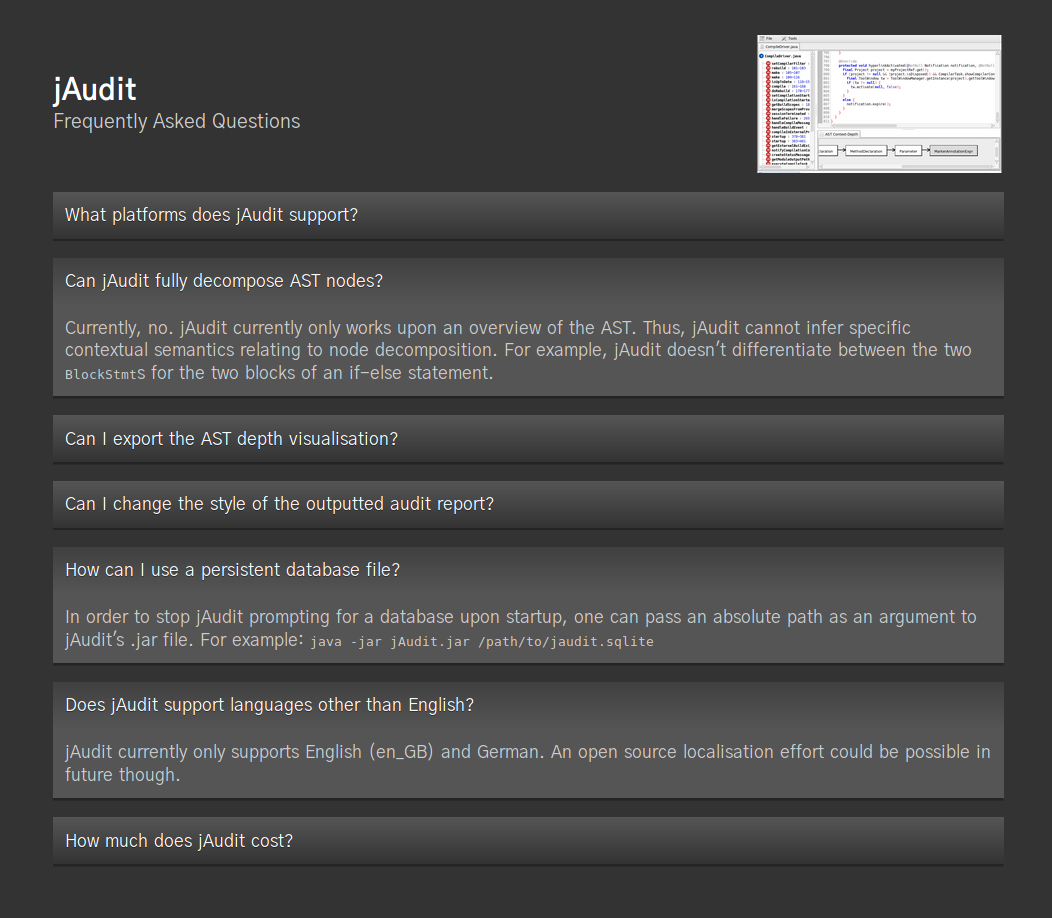
\includegraphics[width=\textwidth]{res/faq.png}
					\caption{FAQ Website}
				\end{figure}
				
				Each question's associated answer can be revealed by simply clicking
				the question - this causes the answer panel to slide down and become
				visible.\\

	\subsection{This Document}
		
		This document can also act as a relevant help guide (or other form of
		documentation) as I believe it outlines motivations, implementation
		details, etc. that could be potentially useful for both users and any
		developers who wish to contribute to jAudit.

\end{document}
